\documentclass{exam}

\usepackage{units} 
\usepackage{graphicx}
\usepackage[fleqn]{amsmath}
\usepackage{cancel}
\usepackage{float}
\usepackage{mdwlist}
\usepackage{booktabs}
\usepackage{cancel}
\usepackage{polynom}
\usepackage{caption}
\usepackage{fullpage}
\usepackage{comment}
\usepackage{enumerate}
\usepackage{xfrac}

\newcommand{\degree}{\ensuremath{^\circ}} 
\everymath{\displaystyle}

\printanswers

% \begin{figure}[H]
%   \centering
%   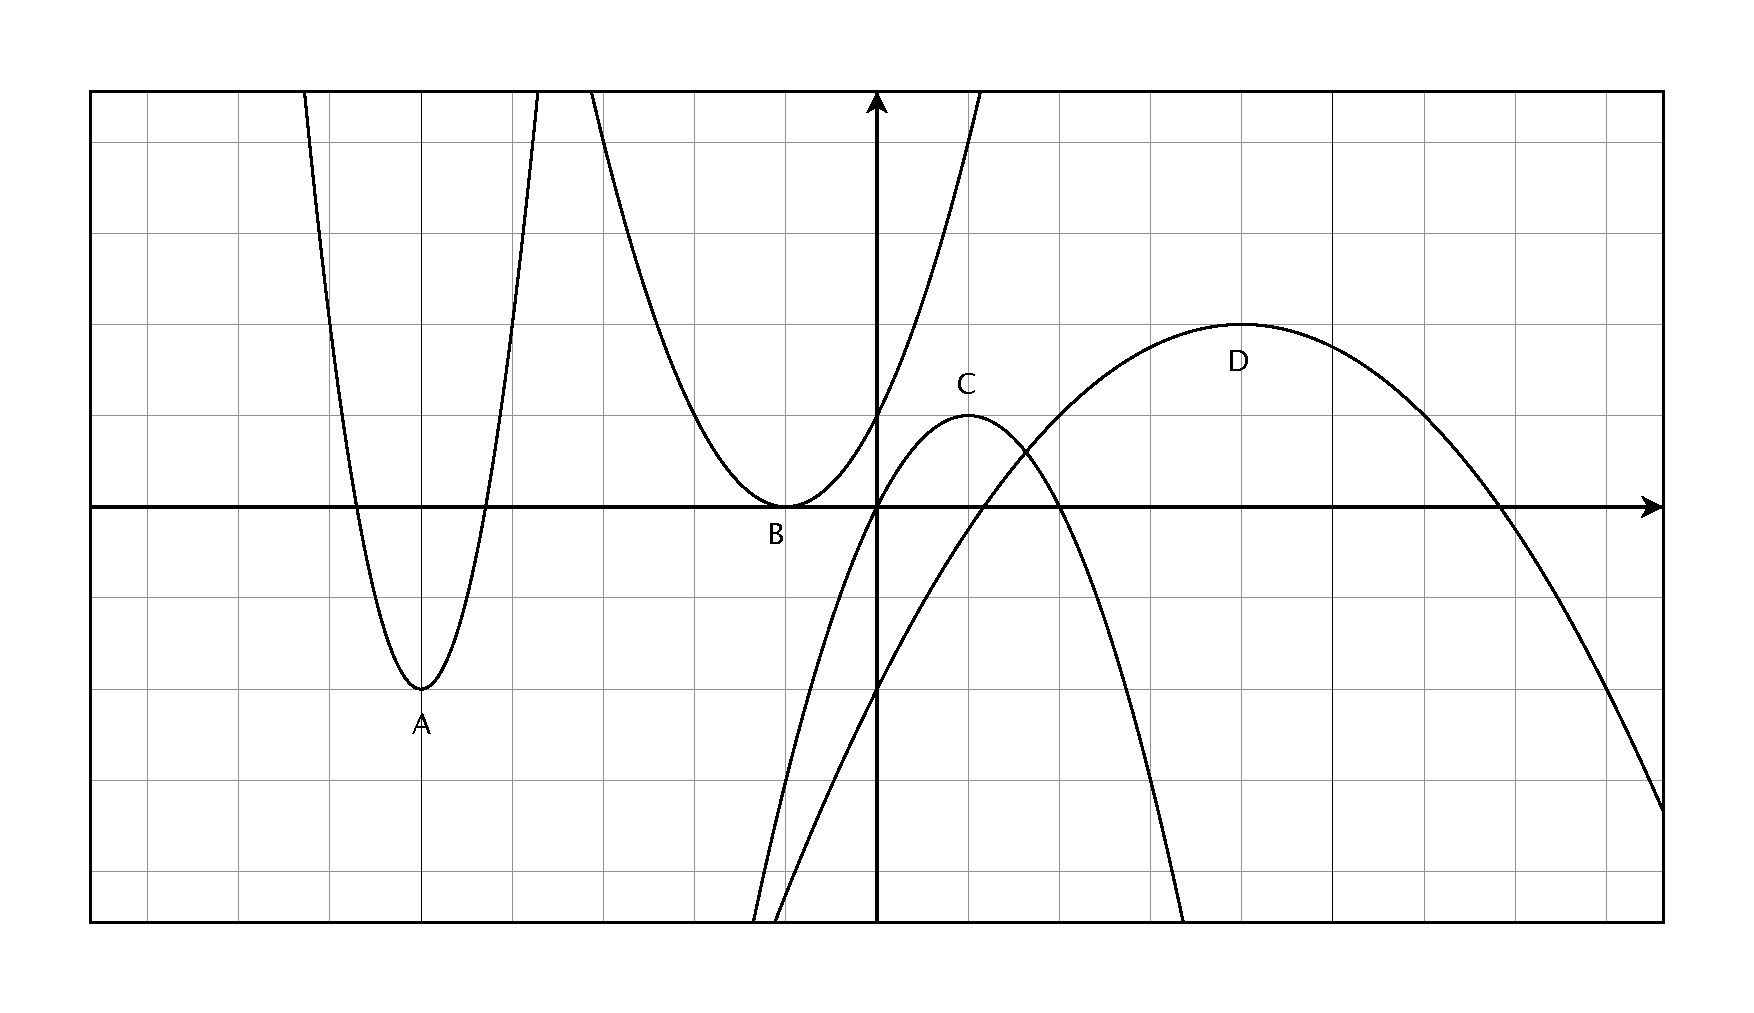
\includegraphics[scale=.3]{problem_7.eps}
%   \caption*{Problem 7}
% \end{figure}

% \begin{tabular}{cc}
% \toprule
% period & amplitude \\
% \midrule
%   $\pi$ & $2$ \\
% \bottomrule
% \end{tabular}

\title{Math 142 Notes \\ Section 5.2}

\date{\today}

\begin{document}

  \maketitle
  \tableofcontents

  \section{Sine/Cosine/Tangent}

  \subsection{Definition}

  On unit circle:
  \begin{itemize*}
    \item sine---y coordinate on unit circle
    \item cosine---x coordinate on unit circle
    \item tangent---$\frac{y}{x}$ ($x \neq 0$)
    \item sine and cosine defined for any value, tangent undefined for $\frac{\pi}{2}$, etc.
  \end{itemize*}

  \subsection{Examples}

  \begin{itemize*}
    \item fill in table with 0, $\pi$, $\frac{\pi}{2}$, $\frac{\pi}{6}$, $\frac{\pi}{4}$, $\frac{\pi}{3}$ (first
      quadrant only)
    \item examples in all quadrants
    \item sign positive in quadrants I and II, etc.
  \end{itemize*}

  \section{Secant/Cosecant/Cotangent}
  \begin{itemize*}
    \item $\frac{1}{x}$, $\frac{1}{y}$, $\frac{y}{x}$
    \item Inverse of sine, etc.
    \item secant undefined for $x = y$, cosecant and cotangent undefined for $y = 0$
    \item show quadrant sign chart for all
  \end{itemize*}

  \section{Evaluating Trigonometric Functions}

  \begin{itemize*}
    \item find reference number
    \item look up from table or memorize
    \item use appropriate sign for quadrant
  \end{itemize*}

  Do examples like $\frac{2 \pi}{3}$, $\frac{5 \pi}{4}$, $- \frac{\pi}{2}$, etc.

  \section{Even/Odd}
  \subsection{Overview}
  \begin{itemize*}
    \item review even/odd definitions
    \item sine, cosecant, tangent, and cotangent are odd

    \item cosine and secant are even

  \end{itemize*}

  \subsection{Examples}
  \begin{itemize*}
    \item $\sin x - \cos x$
    \item $\sin x \cos x$
    \item $x \cos x$ 
  \end{itemize*}

  \section{Identities}

  \subsection{Fundamental Identities}
  \begin{itemize*}
    \item secant, etc. inverses of cosine, etc.
    \item $\sin^2 t + \cos^2 t = 1$
    \item $\tan^2 t + 1 = \sec^2 t$
    \item $\cot^2 t + 1 = \csc^2 t$
  \end{itemize*}

  \subsection{Applications}

  \begin{itemize}
    \item if $\sin t = \frac{2}{5}$ and $t$ is in quadrant II, find the values of the other trigonometric functions
    \item write $\sin t$ in terms of $\cos t$ where $t$ is in quadrant IV, etc.
  \end{itemize}



\end{document}
